\documentclass[../main.tex]{subfiles}
\graphicspath{{subfix{../Images}}}

\begin{document}
\subsection{Data Encryption}
In order to achieve and maintain voter privacy, data published in a publicly accessible ledger needs, at least, a layer of encryption to be applied to it before entering the public structure. This encryption must provide two functionalities: prevent other users from determining the voting options of a specific voter or voters and prevent the calculation of the final tally before the intended process step.
\par
Asymmetrical encryption schemes are a simple and efficient solution for this problem. Our proposed system maintains three essential actors: voters, voting booth contracts, and the tally contract. Each actor can create a pair of asymmetrical keys and distribute the public key, but for our specific case, this task is limited to the smart contracts, i.e., voting both and tally. This removes some complexity from the voter perspective and deposits it into programmable software scripts, which allows for an automation of this process. As such, each voting booth contract and the tally contract generate a pair of asymmetrical encryption keys, with the public key in each one provided to a voter alongside the Vote NFT used to contain their election choices.
\par
Section \ref{multiple_vote_casting} presents a detailed exposition on the encryption scheme.

\subsubsection{Data Obfuscation}
Vote data is double encrypted with the tally contract key and the respective voting booth contract key, i.e., the public encryption key provided by the voting booth contract that mints the Vote NFT requested by a voter. A double encryption scheme increases the solution space for the resulting ciphertexts, which makes a statistical analysis of the encrypted votes harder, but not impossible. In any election, the universe of choices for a given question is finite. If no additional obfuscation methods are employed, especially if any encryption efforts are performed with a small number of encryption keys, the solution space for generated ciphertexts may be small enough to warrant the use of statistical tools that can provide relevant information about the final result before the end of the election.
\par
For example, consider an election that requires a voter to choose one of four choices: \textit{A, B, C, or D}. Consider also a simple encryption scheme that advances the selected option ten positions in the alphabet. With only one encryption layer, the solution space is simply \textit{K, L, M, N}; therefore, determining the final tally without decrypting the vote data becomes a trivial operation in this case. Adding "salt," i.e., a piece of random data, to the plaintext before encrypting it solves this issue by extending the solution space so that statistical analysis is infeasible.
\par
The difficulty of obtaining true random values in a purely deterministic blockchain is well known \cite{Antonopoulos2018}, but for our purpose, a pseudo-random number is sufficient since we are not using it to generate critical system information. Using portions of a hash digest is a popular option to obtain pseudo-random values in a simple and fast fashion. Popular hash functions, such as the ones in the \textit{keccak} family used in the Ethereum blockchain, can be applied to another pseudo-random piece of data, such as the current UNIX timestamp, for example, to obtain these salt values.

\subsubsection{Private Key Management}
The universe of key pairs is equal to the number of smart contracts used to support the election. The transparent nature of these contracts prevents any sensitive information from being published in their code, namely, writing the private keys in the corresponding contracts defeats the whole encryption effort since anyone can check the contract source code and decrypt data stored under it. We solve this problem by relying on the trusted third party that we are already using to determine voter eligibility.

\subsection{Multiple Vote-Casting}
\label{multiple_vote_casting}
Multiple vote-casting is a feature used to combat vote coercion, here defined as someone that can influence how a voter casts his or her choice either through positive (money offers, gifts, etc.) or negative (blackmail, threats of violence, etc.) reinforcement. Vote coercion defeats the purpose of the election. This approach was implemented in e-voting solutions such as the Estonian i-Voting system \cite{Madise2006}, the Norwegian e-Vote project \cite{Barrat2012}, and TiVi, a blockchain-based e-voting solution \cite{TiVi2021}. Voters can submit multiple votes electronically, but only the last one makes the tally. The Estonian i-Voting system, which was deployed in Estonia's 2005 national elections in parallel with a traditional paper ballot system, prioritised the physical vote over the electronic one as well.
\par
The idea behind this approach is to remove incentives from coercers. Even if they are able to "convince" someone to vote against their will, voters always have the opportunity to replace the coerced vote later on or, in the Estonian case, vote physically if they are unable to do so freely from an electronic platform.
\par
We intend to implement a similar, NFT-adapted feature in our proposed solution. The increment in solution complexity is negligible since we already benefit from the fact that we operate with digitally unique NFTs as vote abstractors. In our approach, we considered a strategy based on the replacement of submitted Vote NFTs, i.e., once submitted, the metadata of a Vote NFT cannot be altered, but a submitted token can be replaced by another cast at a later stage, as long as it happens within the voting window defined.
\par
To implement such a feature, we need to ensure the storage strategy used allows for future replacements of submitted tokens while simultaneously ensuring voter and vote privacy, i.e., that any voter information, as well as their choices in the current election, is protected. To ensure privacy along the whole process, the system applies multiple layers of encryption to sensible data, with the public encryption keys shared within the contract code.
\par
The contract stores Vote NFTs using a hash map. The hash value used to index Vote NFTs is calculated before the submission of the Vote NFT, at the user level, where his or her personal information is available and can be prepared such that it produces a unique indexing hash. The usage of already unique identification numbers in this process, such as a National ID number, a Tax Revenue Service ID, Social Security Numbers, etc., ensures this outcome.
\par
Fig. \ref{fig:multiple_vote_casting} represents the full process flow:

\begin{figure}[htp]
    \centering
    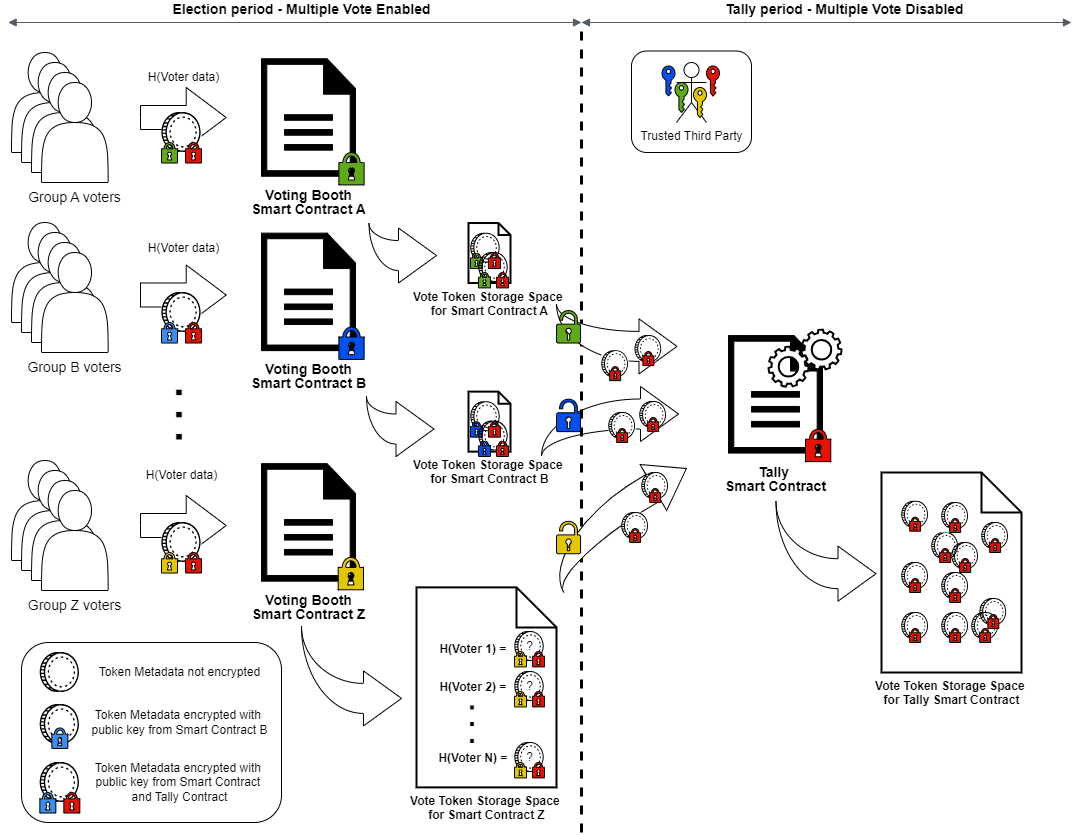
\includegraphics[width=0.8\textwidth]{../Images/MultipleVoteCastingLogic.png}
    \caption{Implementation logic to allow for multiple vote casting.}
    \label{fig:multiple_vote_casting}
\end{figure}


The submission of a Vote NFT also includes a hash digest that is unique for all voters and can be used to retrieve that Vote NFT cast previously by a voter without revealing its contents. During the election period, voting booth contracts store the Vote NFTs. The actual storage location for these tokens is dependent on the blockchain architecture considered, but it is not critical for this explanation.
\par
Double encryption of the vote data by a pair of keys supplied from the voting booth contract and tally contract ensures vote privacy, but the private encryption keys required to decrypt all the voting data need to be securely stored during the whole exercise. A sensible approach is to entrust them to the same trusted third party that ensures the integrity of the list of eligible voters, but other options may be of consideration.
\par
During the election window, users can request and submit multiple Vote NFTs, each replacing any one previously submitted. The link between the tokens and their owners breaks once the voting window closes. This operation also removes the layer of encryption that could be used to divide the tokens per voting booth, thus achieving anonymity between the voters and their choices. The tally contract stores VoteNFT tokens in no specific order.
\par
Removing the last layer of encryption from the token's metadata and computing the final result determines the final tally. Another potential, more private approach consists of computing the tally homomorphically and decrypting only the final result.

\subsection{Security Analysis and Assessment of Threats}
The security of e-voting systems has been the subject of academic research, and it has coalesced around the definition of security criteria, such as voter privacy, transparency, accuracy, etc. The implementation of these criteria through cryptographic features increases the security of the system against dishonest actors. A simple example is using encryption to protect the information in a vote to achieve vote privacy. The number and type of criteria used for this characterisation differ from publication to publication, but some attempts have been made over the years to normalise this exercise. In one of the latest publications dedicated to this effort, \cite{Almeida2023} presented a literature survey that established a series of five criteria deemed "minimal" as the base set from an analysis of a number of publications that employed such characterisation to determine the security offered by the proposed solution.
\par
Alongside this analysis, we also include an assessment of potential threats included in each criterion considered. \cite{Zissi2011} includes a detailed list of potential threats affecting e-voting systems without differentiating between any of the architectural paradigms considered. We adapted this list to our architecture and repeated the threat analysis from the reference point of a decentralised e-voting system.
\par
The following analysis is going to focus on the following security criteria:

\begin{enumerate}

    \item{Accuracy—A voting system is accurate if it does not allow for changes to a vote after submission, changes to the final tally, or invalid votes.}

    \item{Eligibility—Voting systems that allow only registered or valid voters to submit votes implement eligibility.}

    \item{Privacy—A private voting system is able to remove all the links between personal information of the voter and the vote submitted.}

    \item{Verifiability—A voting system is considered verifiable if it allows for independent confirmation of the submission of a vote by the voter.}

    \item{Robustness—A robust voting system is able to prevent and even withstand the actions of dishonest voters to prevent the successful and accurate completion of the voting exercise.}

\end{enumerate}

The framework for minimal security criteria presented in \cite{Almeida2023} provides a framework for security analysis of this proposal.

\subsubsection{Accuracy}
In both approaches considered, once the NFT is written into a block and is part of the chain, the contents of a vote become immutable due to the computational infeasibility of modifying data on the chain.
\par
The final tally is the output from a smart contract function, which adds transparency to the process but does not negate the possibility of an erroneous result or detect any invalid votes. The smart contract uses a function to ensure the correct format of a vote before counting it. Assuming a deterministic computation of the final tally, this means that changes in it imply unauthorised changes to the number of Vote NFTs submitted. An expansion of the previous reasoning negates this scenario as well. Such a change to the number of votes and the number of Vote NFTs stored implies adding and/or removing information from the blockchain, which we have already stated is computationally infeasible.

\paragraph{Threat Assessment}
The accuracy of an e-voting system is affected by adversarial activities such as
\begin{itemize}

    \item{Wiretapping}

    \item{DNS attack}

    \item{Malicious code on client}

    \item{Hardware modification, substitution, and interception}

    \item{Software modification, deletion, edition, trojan horses, information leaks, trapdoors, and viruses}

\end{itemize}

Basing our solution on a blockchain immediately nullifies many of the threats considered above. The immutable and transparent nature of blockchain makes threats based on an adversary being able to alter the system's software and/or hardware irrelevant, as well as any threats from wiretapping communication channels. Deploying software as smart contracts prevents unwanted and undetectable changes to the code. Blockchains also notoriously abstract most hardware characteristics from their overall workings, so as long as nodes execute protocol code as intended, any hardware alterations do not pose a threat.
\par
The most serious threat from this list is the existence of malicious code on a client. The core of the system runs on a distributed, public network, but the submission of individual votes requires an interface that is served from the client side. Realistically, an adversary can replace this interface with a different one without the user noticing it. The risk here is the loss of private information, such as private encryption keys and personal information. If an adversary is able to, for example, control the interface used by someone else to submit votes, such as controlling an unlocked and previously authenticated device (theft, blackmail, threats of violence, etc.), installing remote control software in a device without the owner's permission, etc., he or she can submit a vote under another person's identity. It is difficult to protect the system against such a deep level of control. To counter this threat, the system includes a multiple-vote casting feature. But in the end, the detection of an erroneous submission falls on the voter. The voting booth smart contract provides voting receipts and a history of interactions with the contract itself to ease the detection process. As indicated above, the actions that an adversary has to undertake to be able to cast a vote as someone else can be considered criminal offences with penalties foreseen in most legislative frameworks.

\subsubsection{Eligibility}
\label{voter_eligibility}
The sensible nature of elections prevents the full decentralisation of an e-voting system, at least regarding the presence of a trusted authority that determines the individual eligibility of each voter based on whatever rules exist to regulate a given election (e.g., age, nationality, professional status, etc.). Unless an election is free, i.e., without any regulations regarding who can vote, there is a requirement for a mechanism to implement limitations on the set of voters that are eligible to participate in it.
\par
For our proposal, we consider two approaches to solving this problem in a decentralised fashion:
\begin{itemize}

    \item{Store eligibility information in a centralised database and access it from the blockchain environment using an oracle. Any oracle used for this effect replies to a query in boolean format, i.e., if a voter is (\textit{true})} or is not (\textit{false}) eligible to participate in the election based on the data returned from the centralised database.

    \item{Use a cryptographic accumulator to prove membership in the eligible group of voters. We can use a cryptographic accumulator's properties to infer if a given piece of data related to a specific voter is present in the root value or not. This process is faster and more efficient than checking the existence of a record in a database by searching it exhaustively.}

\end{itemize}

Another possible strategy is used in \cite{Sagar2023}, where the authors used SoulBoundNFTs, a type of non-transferable NFT, for identification purposes. Unfortunately, these NFTs are still in their infancy regarding their development. As such, the present solution omits them. Sections \ref{centralised_eligibility_database} and \ref{cryptographic_accumulators} provide additional details regarding the two approaches considered in determining voter eligibility in our solution.

\paragraph{Oracle Accessible Centralised Eligibility Database}
\label{centralised_eligibility_database}
The basis of our eligibility problem derives from the limitations of current blockchain implementation in storing large quantities of data. Though it is technically possible to do so, storing even a small list of eligible voters directly on the chain is very inefficient, both from an economic (due to potential gas costs) and resource management perspective. This issue is a pertinent one across several application domains.
\par
\cite{Ezzat2022} presents an exhaustive study on strategies proposed to allow blockchain to access off-chain data. Among these, oracles stand out as one of the most promising in terms of flexibility and ease of implementation. Blockchain oracles are implemented as smart contracts that use their functions to query data from the outside, namely by requesting it from an external source, similarly to a regular API. Oracles decrease the gap between blockchains and the external world, which has awarded them the moniker of "blockchain middleware". Cryptocurrency exchanges rely on oracles to allow trades between cryptocurrencies from different blockchains. The value of each tradeable cryptocurrency is currently very volatile and often dependent on speculative factors. Since blockchains themselves do not store the exchange rate of their native token relative to a fiat currency, which is the parameter to consider in inter-blockchain trades, this information is kept instead in "traditional" centralised sources that maintain APIs that can be used to retrieve this information remotely. Oracles are often used in these cases to retrieve the exchange rate of the tokens involved (external information) and provide a fairer exchange of tokens (internal operation).
\par
Oracles fit quite well in our solution. Eligibility data is stored in a conventional, centralised database, and the eligibility state of a given voter is obtained by invoking a function in the smart contract that implements the oracle. Oracles increase the centrality of the solution while potentially creating a point of failure in the system. External data sources do not subject themselves to the blockchain protocol and data redundancy that ensure their integrity; therefore, they can become corrupt with less effort. Therefore, using an oracle in this fashion also requires a trusted third party to ensure the integrity of the external data, which moves this solution away from a purely decentralised one.

\paragraph{Cryptographic Accumulators}
\label{cryptographic_accumulators}
Cryptographic accumulators, also known as set accumulators, are cryptographic primitives that use unidirectional hash functions to represent a set of elements through an \textit{accumulator value}, a single and constant-size value that can be used to determine if a given element belongs to the set without revealing the set contents at any point of the verification process. A hash function $ y = H(x) $ is such that it receives an input $ x $ with arbitrary length to produce a fixed-sized output $ y $, also known as \textit{hash digest}. The unidirectionality of the hash function derives from the fact that

\begin{enumerate}

    \item{For all $ x \in \{0, 1\}^* $ it is computationally easy to calculate $ y = H(x) $.}.

    \item{For all $ y \in \{0, 1\}^n $, it is computationally infeasible to find $ x \in \{0, 1\}^* $ such that $ H(x) = y $.}.

\end{enumerate}

A desirable hash function is also one that provides collision resistance, i.e., it is computationally infeasible to find two input elements, $ x_1, x_2 \in \{0,1\}^* $, such that $ H(x_1) = H(x_2) $, which enables hash digests to be used as data fingerprints, a strategy commonly used to ensure data integrity during communications, software certification during distribution, etc. Among the various use cases of cryptographic accumulators, we highlight \textit{anonymity enhancement} and \textit{identity management} as the most pertinent for our case. Set accumulators can be static or dynamic, depending on their ability to add and remove elements from the original set without requiring the re-calculation of the \textit{cumulative set} \cite{Loporchio2023}. For our particular context, static accumulators are preferable. By publishing the \textit{cumulative value} of the set of eligible voters using a static accumulator, this means that the list of eligible voters "is closed," meaning that, for better or worse, no voters can be added or removed after this publication without changing the \textit{cumulative value} published.
\par
\cite{Benaloh1993} introduced set accumulators as, in a simplistic fashion, the hash digest of the cumulative value of the hash digests of the elements of the set. To determine the \textit{cumulative value} of a set accumulator, one begins by determining the hash digest of every individual element. Individual values are paired and concatenated, and the result rehashed to obtain the values for the next level. The process repeats until a single value—the cumulative value—remains. Fig. \ref{fig:accumulator_example} illustrates this process.

\begin{figure}[htp]
    \centering
    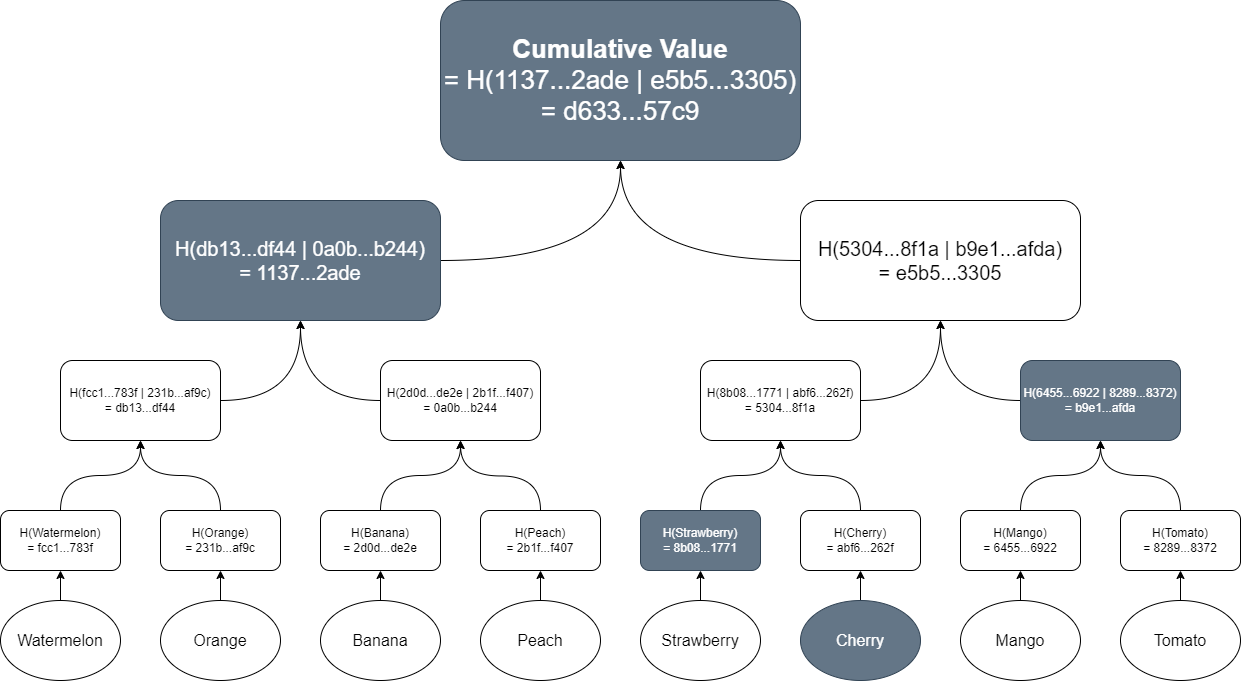
\includegraphics[width=0.8\textwidth]{../Images/AccumulatorExample.png}
    \caption{Simple example of an accumulator to represent a set of strings.}
    \label{fig:accumulator_example}
\end{figure}

An independent verifier can verify the membership of an element by obtaining a minimum of partial results and recalculating the \textit{cumulative value}, starting with the element whose membership he or she desires to verify and combining the successive hashes with the ones provided. If the \textit{cumulative value} matches the one published, the unidirectionality and collision resistance of the hash function ensure that the element does belong to the original set.
\par
Cryptographic accumulators present a solution that benefits from the advantages of storing relevant data directly in the blockchain while keeping that data to a minimum of the required storage space \cite{Wang2021a}. This approach is not novel: in \cite{Chen2020}, the authors use accumulators to optimise a UTXO (\textit{Unspent Transaction Output})-based blockchain by storing the \textit{accumulated value} of the UTXO set in the blockchain instead of the whole set. \cite{Wang2022} apply cryptographic accumulators to authenticate users in an \textit{IoT (Internet Of Things)}-based blockchain, similarly to our proposed strategy.
\par
Our approach is to use a set accumulator to obtain the \textit{cumulative value} of all eligible voters and then use membership functions to determine if a given voter is eligible for the exercise based on the output from the membership function. This eliminates the need to access external data sources while keeping the additional data stored in the chain to a minimum.

\paragraph{Threat Assessment}
% TODO: This fucking part...
\begin{itemize}

    \item{Impersonation}

    \item{Falsification of messages}

    \item{Spoofing}

    \item{Man-in-the-middle Replay attacks}

\end{itemize}

\subsubsection{Privacy}
\label{voter_privacy}
The importance of the storage mechanism is critical to determining how we can achieve voter privacy in the system.
\par
In a contract-based approach, the link between Vote NFT data and the entity that created it is maintained solely in the data structure that maps a specific, unique Vote NFT to an address. The privacy of a voter depends on the difficulty in determining the identity behind these addresses, an issue transversal to all blockchains. It is possible to use statistical tools that analyse blockchain transactions to increase the probability of discovering who is controlling an address, but these often rely on the existence of a significant number of transactions with that address. If a voter uses a specific address solely for voting purposes, this threat diminishes greatly. The pseudo-anonymity of blockchain operations plus the added layer of encryption to the sensible data ensure voter privacy in this system.
\par
Account-based blockchains simplify this by assigning protected storage domains. This ensures that any sensitive operations happen in a cryptographically protected personal space. To gain access to such space, an adversary needs to discover the private counterpart of the asymmetrical encryption key pair used to set up the account, i.e., by breaking an encryption cypher. If the strength of the keys used is sufficiently high, this task should be computationally infeasible, thus also achieving voter privacy within the account-based approach.

\subsubsection{Verifiability}
\label{verifiability}
Implementing this solution in a public blockchain allows us to benefit from transparency regarding the verification of data once it gets written into a block, which in our particular case is in the form of NFT metadata. As with any other NFT published thus far, their contents are open to consultation for anyone, namely, the image, video or audio clip, text, etc., that got encoded into that NFT. Unfortunately, this level of transparency also defeats any attempts to keep voter data private, thus negating the \textit{Privacy} feature described in Section \ref{voter_privacy}. But as it was also indicated in this section, any sensible data written into the public blockchain (regardless of the storage approach considered) needs to be protected to implement even the weakest form of voter privacy. This opens up two practical approaches to implementing vote verifiability:

\begin{enumerate}
    \item{If a vote is published after being encrypted using public encryption keys whose private counterparts are being carefully controlled by a trusted third party, as suggested in Section \ref{contract-based-approach}, a voter can verify the correct submission of his or her vote by comparing the ciphertext in the metadata for the Vote NFT associated with his or her address (this is valid for both contract and account-based storage approaches) to the result of a re-encryption of his or her original vote. The voter is unable to decrypt the data directly in the Vote NFT metadata because that would require knowledge of the private encryption keys, which are kept secure by a trusted third party. A voter is able to verify his/her vote at a later stage simply by replicating the data encryption process. If the result matches the value in the blockchain, the vote remains unchanged. This approach requires the use of "salt" to prevent an adversary from executing the same exercise, as mentioned previously in Section \ref{sec:data_obfuscation}. This strategy mimics others used to establish secure communications over insecure channels, as detailed in \cite{Merkle1978} and \cite{Merkle1980}}.

    \item{A simpler and more practical alternative is to "fingerprint" vote data with a hash digest, using all data present in the Vote NFT metadata, for example, and including it as another parameter in the Vote NFT. Like the previous approach, voters can ensure that their vote remains unchanged after submission by re-creating the vote and re-hashing it. If the digest obtained this way matches the one written on-chain via the Vote NFT's metadata, the encoded vote is exactly the same as the one just reproduced. This also opens the possibility of an adversary using this method to break the privacy of voters. If an adversary knows the format used and sufficient personal data from a voter, he or she can determine the voter's choices by obtaining the hash digest written in the submitted Vote NFT metadata, by brute force if needed. As such, the use of "salt" or any other parameter exclusive to the knowledge of the voter needs to be used to ensure vote verifiability without compromising vote privacy.}
\end{enumerate}

\subsubsection{Robustness}
\label{robustness}
Blockchain-based systems benefit directly from the security they derive from the cryptographic methods they use to establish basic data integrity. The effort required to change the value of a vote or the final tally is as computationally infeasible as manipulating a block of transactions in a double-spending attempt.
\par
Determining voter eligibility with an external database, through an oracle, for example, is a potential source of corruption. Any off-chain elements are, by definition, weak points of a decentralised system since they represent an exception in the paradigm. This threat can be mitigated by the use of hash digests of the list of voters and their data, published once a valid and final list is achieved and verified periodically to detect unwanted modifications.

\end{document}.